\section{Filtraggio dei dati}

Una volta ottenuti i dati, l'applicazione \textit{client-side} \idest{lo script
JavaScript \code{dati-storici.js}} può opzionalmente filtrarli per stazione o
per inquinante. Due drop-down list forniscono all'utente la lista di tutte le
stazioni presenti nella provincia selezionata e tutti gli inquinanti per i quali
sono disponibili misurazioni.

Per filtrare per inquinante, è sufficiente utilizzare solo i dati aggregati
relativi all'inquinante selezionato dall'utente per riempire i valori della
tabella e del grafico Google Charts. Di questo si occupa la funzione
\code{changingPollutantFilter()}.

Per filtrare invece per stazione non possiamo utilizzare i dati aggregati in
quanto non contengono le informazioni sulle stazioni che hanno effettuato le
misurazioni. Pertanto, quando l'utente seleziona una stazione dalla lista, è
necessaria una nuova richiesta AJAX POST al server che esegue la query seguente
per ottenere i dati per la sola stazione selezionata.

La query è eseguita dallo stesso script \code{getHistoricalData.php} che
discrimina le richieste di dati aggregati per provincia o per singola stazione
in base a quali parametri POST vengono utilizzati nella richiesta.

La query ha buone performance in questo caso, dato che deve prelevare i dati di
una singola stazione e non di tutte le stazioni di una provincia, quindi anche
il numero di misurazioni totali è molto ridotto.

In seguito al filtraggio (sia per stazione che per inquinante) il codice
JavaScript utilizza una struttura dati identica a quella utilizzata per i dati
non filtrati. Pertanto possiamo sfruttare il riutilizzo del codice per mostrare
i dati nella tabella e nel grafico.

In Figura \vref{fig:filtering} è mostrato un esempio di filtraggio sia per
stazione che per inquinante per la provincia di Pisa.

\begin{figure}[p]
	\centering
	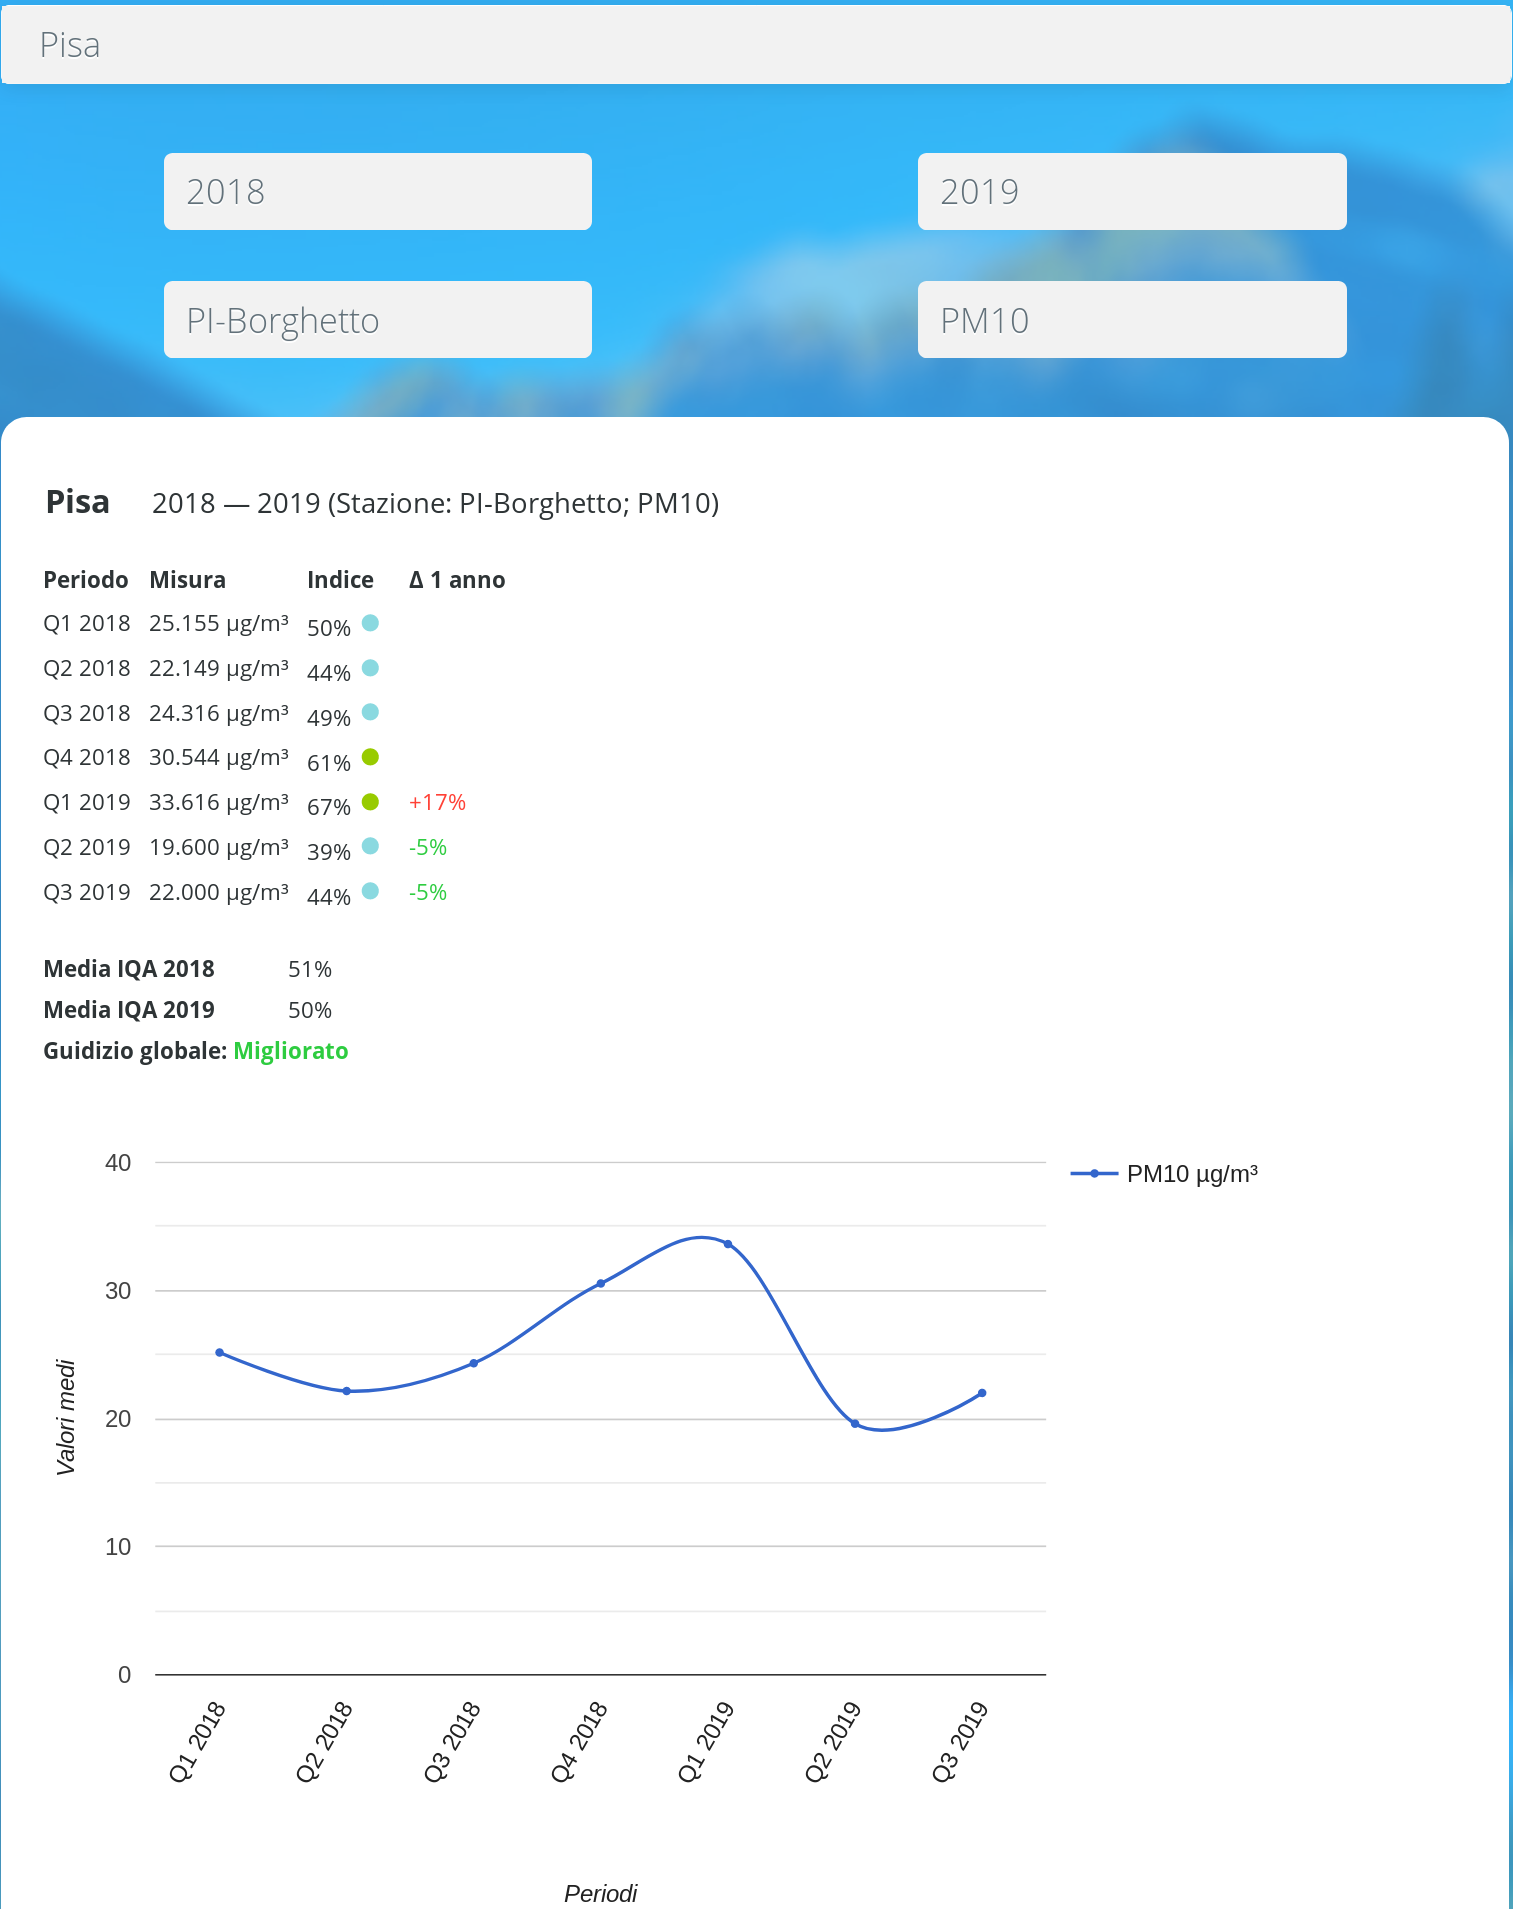
\includegraphics[width=\textwidth]{img/filtering}
	\caption{Esempio di filtraggio per stazione e per inquinante per la
	provincia di Pisa.}\label{fig:filtering}
\end{figure}
